\documentclass[ twocolumn,notitlepage]{ revtex4-1}
\input{header.txt}
\begin{document}
\title{Area and Eccentricity of Fibroblasts During Trypsinization}\author{Kyle Thomas}\date{\today}\maketitle

\begin{abstract}
\begin{center}
Area and eccentricity of mouse-embryo fibroblast cells are both measured as the cells release the top surface of collagen gel. Image sets of the cells are collected at regular time-intervals during and after detachment. Software was written to segment selected cells and measure both the area and eccentricity of each segmented cell. Some code is included in appendices as well as a link to all of the code.
\end{center}
\end{abstract}

\section*{Experiment Methods}
\begin{figure}
  \centering
  \caption{Orange cells submerged in violet growth medium atop green collagen are diagrammed.}
  \includegraphics[clip=true,width=.4\textwidth]{img/cells-diagram}
  \label{fig:cellDiagram}
\end{figure}

Mouse embryo fibroblasts exhibiting green fluorescent protein (cell line NIH3T3/GFP) are placed atop a collagen-gel and suspended in growth medium(see the diagram in Figure \ref{fig:cellDiagram}). The fibroblasts attach to the surface of the collagen at 37$^\circ$C for 15 to 30 hours in a CO2-regulated incubator. The cells were not seen to undergo mitosis.

Cells are imaged every regularly beginning 40 minutes before trypsinization via TrypLE Select. The images are collected with a confocal microscope using a 70/30 transmission/reflection beam-splitter. The images are collected in image sets called z-stacks.

A z-stack is a sequence of images taken in quick succession. After the first, lowest image, each image is focused a few microns higher than the preceding image. Imaged in this way, z-stacks essentially provide a "snapshot" of the state of specific cells within the sample.

The stage is adjusted before imaging a sample so that the z-stacks image from ten microns below the surface of the collagen to ten microns above the surface of the collagen. Ten microns is approximately the radius of these cells when not attached to the collagen. Z-stacks are captured every five to fifteen minutes.

Imaging the cells occurs by irradiating the sample with a 488nm laser. The green fluorescent proteins fluoresce at a different wavelength than the 488nm excitation light, thereby distinguishing fluorescence from reflection. Light from 500nm to 550nm is observed for emissions of the GFP. 

The fibers were also observed for alignment phenomena which were not seen.To image the fibers, the sample is excited by a 532nm laser and wavelengths in the spectrum 531nm to 536nm are observed for reflection and transmission of the incident light off of the fibers. The observation spectrum imaged for the fibers was found by visually determing the spectrum in which the fibers appear most distinct.

Light detected from the fibers is maximized by observing a spectrum symmetric about the wavelength of the incident light, say 526nm to 536nm. However, such a spectrum has a higher signal to noise ratio because more of the light emitted by the GFP is detected below 531nm.

Both sets of images are acquired with a 30\% reflection, 70\% transmission beamsplitter. Using the same beamsplitter for both images means time is not spent changing the beamsplitter between images. This time savings between frames allows a z-stack to be captured closer to instantaneously. An instantaneous "snapshot" of the z-stack is ideal. 

During imaging, the growth-medium surrounding the cells is rinsed with 1XPBS twice. The PBS is next replaced with TrypLE Select. The TrypLE Select breaks the proteins binding the cells to the collagen-matrix.

The proteins that bind the cells to the collagen are on bulges in the cell-membrane. These protrusions are called filopodia. After the bonds break, these filopodia flatten back into the cells.

This flattening of the philopodia leaves the cells somewhat spherical. The spherical fibroblasts appear as circles when seen through the microscope. While the cells return to a spherical shape, their lack of sphericilaty can be measured as eccentricity, as in the eccentricty of an ellipse.

\section*{Image Processing Methods}
A single experiment produces a folder containing all the z-stacks acquired during the experiment. Each z-stack is comprised of several images, as described before. The image files for a z-stack are combined into a single TIFF using Matlab. A maximal intensity projection is used to transform all images comprising a z-stack into a single image.

The Matlab function mip creates a maximal intensity projection for each z-stack. This maximal intensity projection is a single image. The maximal intensity projection is made by using the value of the brightest pixel at position $(x_1,y_1)$ of every image in the image's z-stack. An example MIP-creation process is shown in Figure \ref{fig:mip-illustration}.

\begin{figure}[!h]
%\centering
\includegraphics[width=.4\textwidth]{./img/mip-illustration.pdf}
\caption{The mip function is illustrated projecting simple example images.}
\label{fig:mip-illustration}
\end{figure}

The function maskmaker is used to draw a region loosely enclosing a single cell at its most stretched out. Maskmaker sets pixels outside the region to black. This creates a mask loosely surrounding the cell of interest. Applying this mask leaves the user-selected cell as the largest object in the image so that the segmentation of the selected cell can proceed. 

The function stackmasker applies this mask to all images in the stack. All masked images contain the entire cell of interest. The mask is drawn around the cell when the filopodia are stretched out to ensure the whole cell is visible in later images as the cell's filopodia recede.

Masking works by ensuring that the cell of interest is the largest object shown. A mask is made loosely enclosing a single cell so that the user can specify a certain cell for software to outline precisely. Cells are precisely outlined by software to save time and to ensure uniformity in drawing outlines.

Filling the objects in the image proceeds as follows. The brightness of each masked image is multiplied by a constant factor. This factor is 15 by default for the trypsinization images. Some z-stacks were brightened by a factor of more than 15 to facilitate masking entire cells.

The Matlab Image Processing Toolbox function im2bw uses a brightness threshold to create a black and white image from a grayscale image. Pixels brighter than the threshold value are converted to white while other pixels are turned to black. The threshold used to create binary(black and white) images is 0.15.

Several experiments show multiple cells in each image. For example, consider an image that contains cells A and B. Each cell's shape and eccentricity can be measured separately. 

A cell is measured by creating a separate binary set of images for that cell. The cell is segmented by ensuring it is the only object visible in its image-set.

Cell A is loosely masked by the user so that it's the largest object visible. Cell A is segmented in the images. These images showing only cell A are saved. The area and eccentricity of cell A is measured from these images. This process is repeated to measure cell B.

Image segmentation yields multipage-tiff-files, where each page is a 1024 pixel by 1024 pixel image. All images in a file show only the same particular cell. The images are taken 20 minutes apart so that each file watches a different cell as it releases the collagen substrate.

%\section*{Conclusions}
%
%\section*{Acknowlegements}
%
%\section*{References}

\newpage\section*{Appendices}
\subsection*{Appendix A: Experiment Protocol}
The protocol for three collagen-samples of concentration 1.5 and gelled at 21$^{\circ}$C is as follows:
\begin{enumerate}
	\item Create the collagen-solution.
	\begin{enumerate}
		\item Total volume to be made is V = (90$\mu$L per sample)(3 samples)(150\%) = 405$\mu$L.
		\item Combine 40.5$\mu$L 10X PBS, 14.2$\mu$L NaOH, and 276.3$\mu$L growth-medium.
		\item Shake this solution at 400rpm for 20 seconds.
		\item Store at 6$^{\circ}$C for 10 minutes.
		\item Add 71$\mu$L collagen homogeneously.
		\item Stir collagen into solution with a 100$\mu$L pipette tip.
		\item Pipette 90$\mu$L collagen-solution into each of the 3 samples a, b, and c.
		\end{enumerate}
	\item Wrap each sample in film and let gelate at 21$^{\circ}$C for two hours.
	\item Place growth-medium on all samples and place cells on sample a.
	\item Place cells on sample b four hours later.
	\item Place cells on sample c four hours later.
	\item Using confocal fluorescence microscopy, capture a 10$\mu$m tall z-stack of images of fibers and cells, separately, every 20 minutes for four hours.
	\begin{enumerate}
		\item After the first z-stack, replace the growth-medium on the sample with 1X PBS.
		\item After the second z-stack, replace the PBS with fresh PBS.
		\item After the third z-stack, replace the PBS with 1X TrypLe\texttrademark\hspace{.1em} Select.
	\end{enumerate}
		\item When sample a is finished imaging, image sample b in the same way as sample a was imaged.
		\item When sample b is finished imaging, image sample c in the same way as sample a was imaged.
\end{enumerate}

\newpage
\begin{widetext}
\subsection*{Appendix B: Code}
\lstinputlisting[ language=Matlab,
                  caption=segmenter.m,
                  label=segmenter ]
                {./matlab/original/segmenter.m}

\newpage
\lstinputlisting[ language=Matlab,
                  caption=regionPropsScript.m,
                  label=regionPropsScript ]
            {./matlab/original/regionPropsScript.m}

\newpage          
\lstinputlisting[ language=Matlab,
                  caption=plotterScript.m,
                  label=plotterScript ]
                {./matlab/original/plotterScript.m}
\end{widetext}
\end{document}
